% =====================================================================
% Relatório do Trabalho de Computação Gráfica, 2ª etapa (2026.2)
% Compilar: latexmk  (ou pelo Overleaf, com o compilador pdfLaTeX)
% Cada seção fica em um arquivo separado dentro de secoes/
% =====================================================================
\documentclass[12pt,a4paper]{article}
% =====================================================================
% Preâmbulo: formatação do relatório (base ABNT, mesmo modelo do SAACI)
% Não mexer aqui sem combinar com o grupo.
% =====================================================================

% --- Idioma e codificação ---
\usepackage[T1]{fontenc}
\usepackage[utf8]{inputenc}
\usepackage[brazilian]{babel}
\usepackage{csquotes}

% --- Fonte: Times New Roman 12 ---
\usepackage{mathptmx}
\usepackage{microtype}

% --- Página A4, margens: sup. e esq. 3 cm; inf. e dir. 2 cm ---
\usepackage[a4paper,top=3cm,left=3cm,bottom=2cm,right=2cm,headsep=0.6cm,headheight=15pt]{geometry}

% --- Espaçamento 1,5 e parágrafo com recuo de 1,25 cm, justificado ---
\usepackage{setspace}
\onehalfspacing
\usepackage{indentfirst}
\setlength{\parindent}{1.25cm}
\setlength{\parskip}{0pt}

% --- Número de página no canto superior direito ---
\usepackage{fancyhdr}
\pagestyle{fancy}
\fancyhf{}
\fancyhead[R]{\thepage}
\renewcommand{\headrulewidth}{0pt}
\fancypagestyle{plain}{\fancyhf{}\fancyhead[R]{\thepage}\renewcommand{\headrulewidth}{0pt}}

% --- Títulos de seção: "1. Introdução", em negrito ---
\usepackage{titlesec}
\renewcommand{\thesection}{\arabic{section}}
\renewcommand{\thesubsection}{\arabic{section}.\arabic{subsection}}
\renewcommand{\thesubsubsection}{\arabic{section}.\arabic{subsection}.\arabic{subsubsection}}
\titleformat{\section}{\normalfont\fontsize{13}{15}\bfseries}{\thesection.}{0.4em}{}
\titleformat{\subsection}{\normalfont\normalsize\bfseries}{\thesubsection}{0.5em}{}
\titleformat{\subsubsection}{\normalfont\normalsize\bfseries}{\thesubsubsection}{0.5em}{}
\titlespacing*{\section}{0pt}{18pt}{6pt}
\titlespacing*{\subsection}{0pt}{12pt}{4pt}
\titlespacing*{\subsubsection}{0pt}{10pt}{4pt}

% --- Figuras, tabelas e quadros: legenda ACIMA, fonte ABAIXO, tamanho 10 ---
\usepackage{graphicx}
\usepackage{float}
\usepackage{booktabs}
\usepackage{tabularx}
\usepackage[font={footnotesize,singlespacing},labelsep=endash,justification=centering,skip=4pt]{caption}
\usepackage{subcaption}
\captionsetup[figure]{name=Figura,position=above}
\captionsetup[table]{name=Tabela,position=above}
\captionsetup[sub]{labelformat=parens,labelsep=space,position=below}

% Quadro (texto, bordas fechadas): ambiente próprio, numeração própria
\usepackage{amsmath}
\usepackage{newfloat}
\DeclareFloatingEnvironment[fileext=loq,name=Quadro,placement=H]{quadro}
\captionsetup[quadro]{position=above}

% Diagramas desenhados no próprio LaTeX (câmera, volume de visão, Phong, retas, scan line, baricêntrica)
\usepackage{tikz}
\usetikzlibrary{arrows.meta,calc}

% \fonte{...}: linha "Fonte: ..." abaixo de figura, tabela ou quadro
\newcommand{\fonte}[1]{\par\vspace{2pt}{\centering\footnotesize Fonte: #1\par}}

% \figura{arquivo}{largura}{legenda}{rótulo}{fonte}
\newcommand{\figura}[5]{%
  \begin{figure}[H]
    \centering
    \caption{#3}\label{#4}
    \includegraphics[width=#2]{#1}
    \fonte{#5}
  \end{figure}}

% Caminho das imagens
\graphicspath{{figuras/}}

% --- Listas ---
\usepackage{enumitem}
\setlist{nosep,leftmargin=1.25cm}

% --- Citação direta longa: recuo de 4 cm, fonte 10, espaço simples, sem aspas ---
\newenvironment{citacao}{%
  \par\vspace{6pt}\begin{list}{}{\setlength{\leftmargin}{4cm}\setlength{\rightmargin}{0pt}}
  \item[]\footnotesize\singlespacing}{%
  \end{list}\vspace{6pt}}

% --- Referências ABNT (NBR 6023:2018) com biblatex-abnt ---
\usepackage[style=abnt,backend=biber,justify=false,extrayear]{biblatex}
\addbibresource{referencias.bib}
% NBR 10520:2023: no texto, autor só com a inicial maiúscula -> (Martin, 2017).
% Na lista de referências o SOBRENOME continua em CAIXA ALTA.
\makeatletter
\renewcommand*{\UpperOrSCCite}[1]{#1}
\DeclareFieldFormat{uppercasecite}{#1}
\makeatother
\setlength\bibitemsep{\baselineskip}
\renewcommand*{\bibfont}{\normalsize\singlespacing}

% --- Links (sem caixas coloridas) ---
\usepackage[hidelinks]{hyperref}
\urlstyle{same}

% --- Comando para marcar o que falta confirmar (aparece em vermelho) ---
\usepackage{xcolor}
\newcommand{\confirmar}[1]{\textcolor{red}{[CONFIRMAR: #1]}}
% Para a versão final: descomente a linha abaixo para esconder as marcações
% \renewcommand{\confirmar}[1]{}


\begin{document}

% Capa (sem número de seção)
% =====================================================================
% Capa (NBR 14724) e sumário. Sem número de seção.
% =====================================================================
\begin{titlepage}
  \thispagestyle{empty}
  \centering
  \singlespacing

  {\bfseries INSTITUTO FEDERAL DE EDUCAÇÃO, CIÊNCIA E TECNOLOGIA DO CEARÁ\par
  CAMPUS FORTALEZA\par
  DEPARTAMENTO DE TELEMÁTICA\par
  CURSO DE ENGENHARIA DA COMPUTAÇÃO\par}

  \vspace{1.5cm}

  {\bfseries \confirmar{nome do aluno 1}\par
  \confirmar{nome do aluno 2}\par
  \confirmar{nome do aluno 3}\par}

  \vfill

  {\fontsize{16}{19}\selectfont\bfseries \confirmar{título do trabalho}\par}
  \vspace{6pt}
  {\large Computação Gráfica: Trabalho da 2ª etapa\par}

  \vfill

  \begin{flushright}
    \begin{minipage}{0.5\textwidth}
      \small\raggedright
      Relatório apresentado à disciplina de Computação Gráfica do curso de Engenharia da Computação do IFCE, campus Fortaleza.\par
      \vspace{6pt}
      Professor: Ajalmar Rocha Neto, Dr.
    \end{minipage}
  \end{flushright}

  \vfill

  {\bfseries Fortaleza\par
  2026\par}
\end{titlepage}

\tableofcontents
\clearpage


% =====================================================================
% 1. Introdução
% =====================================================================
\section{Introdução}\label{sec:introducao}

O pipeline gráfico é a sequência de etapas que transforma objetos 3D em uma imagem 2D: modelagem,
composição da cena, câmera, projeção, iluminação e rasterização \cite{azevedo2018}.
\confirmar{edição, ano e editora do livro Azevedo; Conci; Vasconcelos} Neste trabalho, o grupo
percorreu todas as etapas com cinco objetos do cotidiano: lápis, peão de xadrez, haltere, martelo e
lixeira. Cada objeto foi descrito por uma função matemática e convertido em malha de triângulos com
o algoritmo \textit{Marching Cubes} \cite{lorensen1987}. A cena foi vista por uma câmera,
projetada em perspectiva, iluminada pelo modelo de Phong \cite{phong1975} e rasterizada por um
rasterizador implementado pelo grupo.

O código foi escrito em Python. A biblioteca NumPy \cite{harris2020} cuidou das operações com
matrizes, e a Matplotlib \cite{hunter2007} exibiu as imagens. Apenas o \textit{Marching Cubes}
veio pronto, da biblioteca scikit-image \cite{vanderwalt2014}. As demais etapas foram
implementadas pelo grupo.

% =====================================================================
% 2. Objetivos
% Dica: um objetivo geral e os específicos, seguindo os itens 1 a 6 do enunciado.
% =====================================================================
\section{Objetivos}\label{sec:objetivos}

\subsection{Objetivo geral}\label{sec:obj-geral}

\confirmar{escrever: objetivo geral em uma ou duas frases}

\subsection{Objetivos específicos}\label{sec:obj-especificos}

\confirmar{ajustar a lista abaixo ao que foi entregue}

\begin{itemize}
  \item modelar cinco objetos do cotidiano como malhas de triângulos com normais para fora;
  \item compor uma cena no sistema de coordenadas do mundo, sem sobreposição e dentro do limite $|10|$;
  \item transformar a cena para o sistema de coordenadas da câmera;
  \item projetar a cena em perspectiva na janela de projeção;
  \item calcular a iluminação (ambiente, difusa e especular) nos vértices visíveis;
  \item rasterizar os polígonos em três resoluções, com interpolação baricêntrica.
\end{itemize}

% =====================================================================
% 3. Desenvolvimento
% Uma subseção por etapa do enunciado (itens 1 a 6). Cada uma fica em um arquivo
% em secoes/03-desenvolvimento/ e as imagens em figuras/03-desenvolvimento/<etapa>/.
% =====================================================================
\section{Desenvolvimento}\label{sec:desenvolvimento}

Esta seção explica cada passo do trabalho, na mesma ordem do enunciado: criar os objetos, montar
a cena, colocar a câmera, projetar em perspectiva, calcular a luz e pintar a imagem. O código foi
separado em arquivos, e cada arquivo cuida de uma parte, como mostra a
Tabela~\ref{tab:arquivos}.

\begin{table}[H]
  \centering
  \caption{Arquivos do código e suas funções}\label{tab:arquivos}
  \begin{tabularx}{\textwidth}{lX}
    \toprule
    Arquivo & O que faz \\
    \midrule
    \texttt{primitives.py} & formas simples (cilindro, esfera, caixa, etc.) e como juntá-las \\
    \texttt{modeling.py} & cria a malha de triângulos e define os cinco objetos \\
    \texttt{math\_3d.py} & matrizes de translação, escala, rotação, câmera e projeção \\
    \texttt{illumination.py} & cálculo da luz pelo modelo de Phong \\
    \texttt{rasterizer.py} & desenho de retas, preenchimento dos triângulos e cores \\
    \texttt{main.py} & monta a cena, roda todos os passos e mostra as imagens \\
    \bottomrule
  \end{tabularx}
  \fonte{Os autores (2026).}
\end{table}

% Etapa 1 do enunciado: modelagem dos 5 objetos.
% Fonte no código: primitives.py, modeling.py
% Função que retorna o sólido: modeling.criar_solido. Figuras: visualizar_objetos.py (salvas pelo botão de salvar da janela).
\subsection{Modelagem dos objetos}\label{sec:modelagem}

Os cinco objetos foram modelados cada um no seu sistema de coordenadas, apoiados em $y = 0$ e
centrados no eixo $y$. Só o haltere fica deitado, ao longo do eixo $x$.

Cada objeto é uma função $F(x, y, z)$ que vale menos que zero dentro do objeto, zero na superfície e
mais que zero fora. Formas simples (cilindro, cone, esfera, caixa e toro) são combinadas: a união é
o mínimo entre as funções e a subtração é $\max(A, -B)$, usada para deixar a lixeira oca. O
algoritmo \textit{Marching Cubes} \cite{lorensen1987}, da biblioteca scikit-image
\cite{vanderwalt2014}, recebe $F$ em uma grade de 80 pontos por eixo e devolve os triângulos de
$F = 0$.

A função \texttt{criar\_solido} devolve vértices, faces, arestas, normais das faces, normais dos
vértices e cor, tudo em coordenadas do objeto. As normais apontam para fora. Em todos os objetos, a
malha satisfaz $V - A + F = 2$, o que indica superfície fechada e sem buracos. A
Figura~\ref{fig:objetos} mostra os objetos com os eixos e as normais de algumas faces (setas
pretas), em uma grade de 50 pontos por eixo, mais leve para exibir. A cena usa 80 pontos.

\begin{figure}[H]
  \centering
  \caption{Objetos no sistema de coordenadas do objeto}\label{fig:objetos}
  \begin{subfigure}{0.31\textwidth}
    \centering
    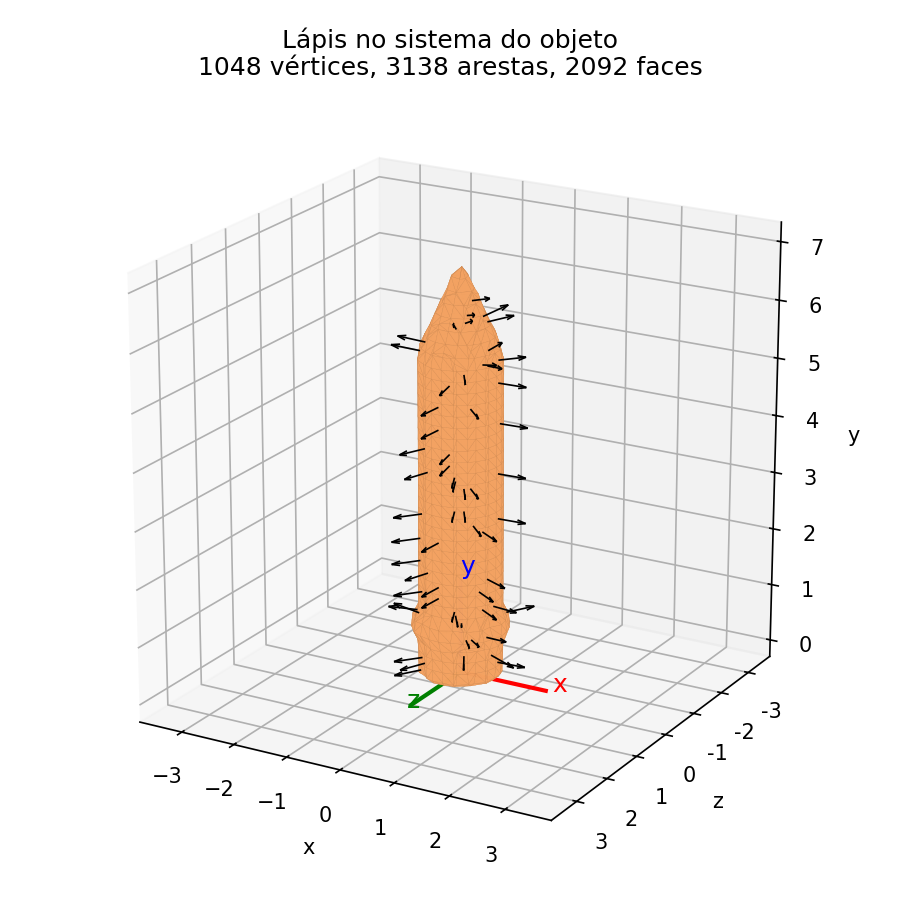
\includegraphics[width=\textwidth]{03-desenvolvimento/01-modelagem/lapis.png}
    \caption{Lápis}
  \end{subfigure}\hfill
  \begin{subfigure}{0.31\textwidth}
    \centering
    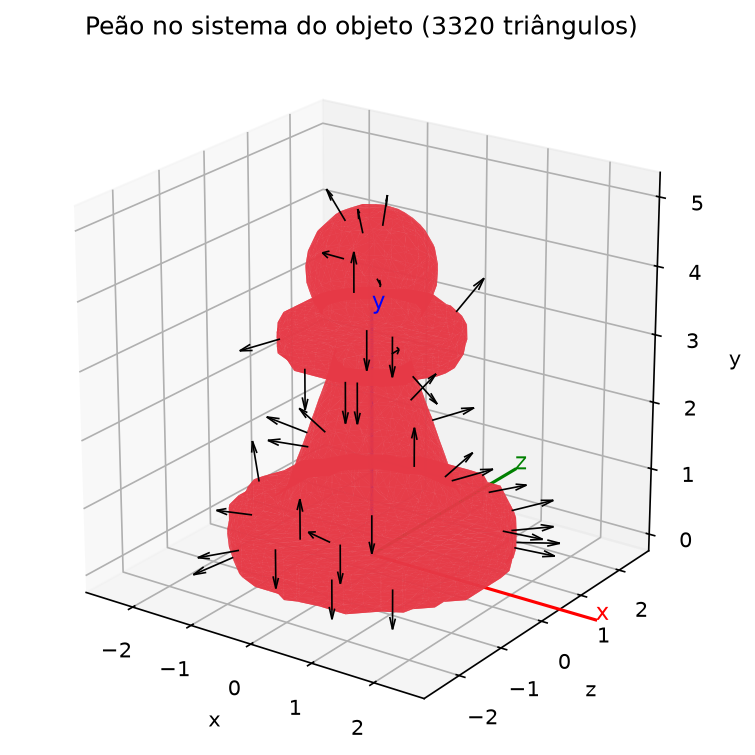
\includegraphics[width=\textwidth]{03-desenvolvimento/01-modelagem/peao.png}
    \caption{Peão}
  \end{subfigure}\hfill
  \begin{subfigure}{0.31\textwidth}
    \centering
    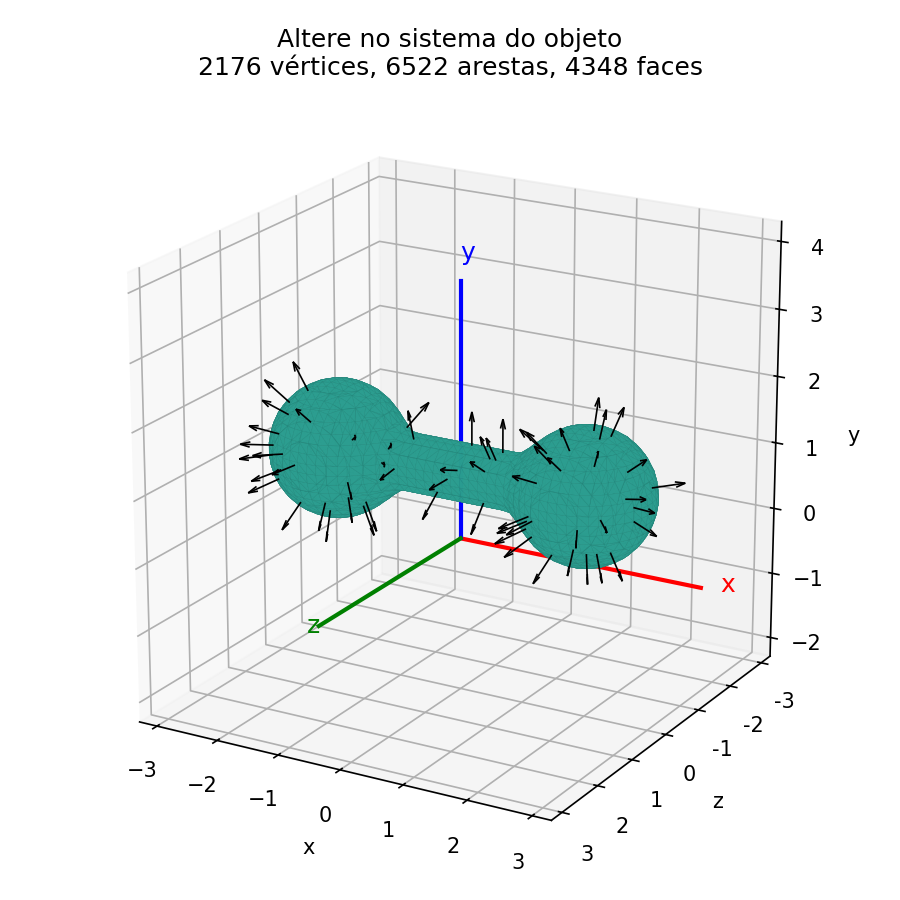
\includegraphics[width=\textwidth]{03-desenvolvimento/01-modelagem/haltere.png}
    \caption{Haltere}
  \end{subfigure}

  \vspace{6pt}
  \begin{subfigure}{0.31\textwidth}
    \centering
    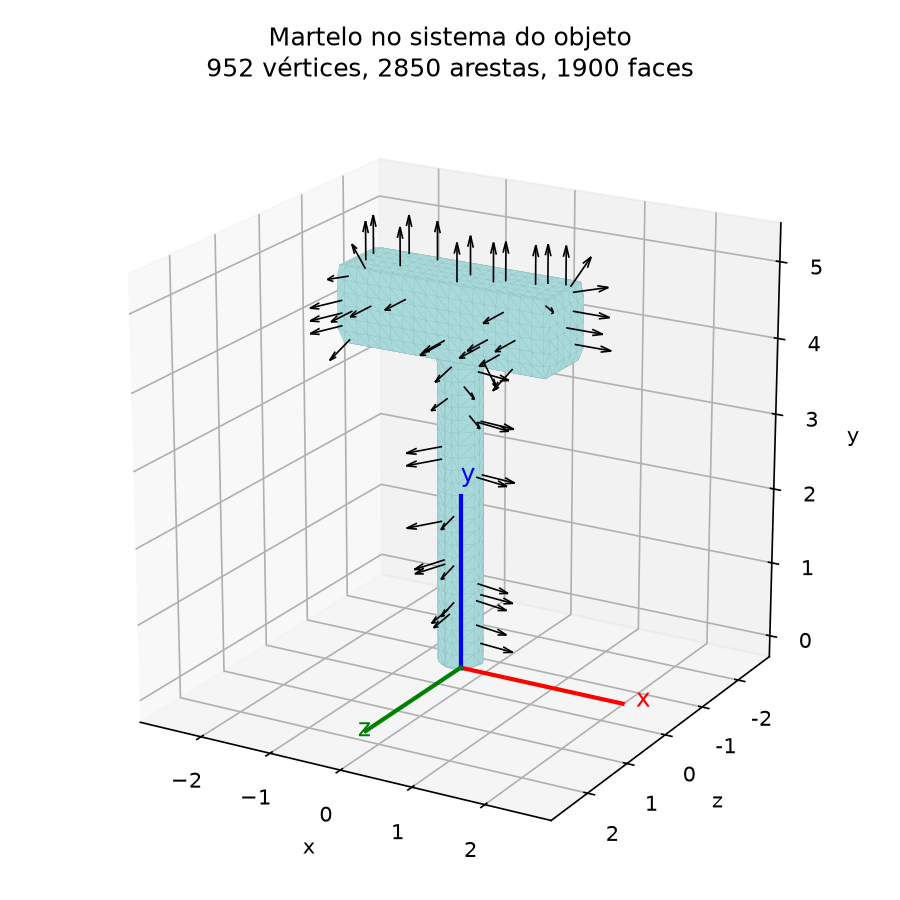
\includegraphics[width=\textwidth]{03-desenvolvimento/01-modelagem/martelo.png}
    \caption{Martelo}
  \end{subfigure}\hspace{0.04\textwidth}
  \begin{subfigure}{0.31\textwidth}
    \centering
    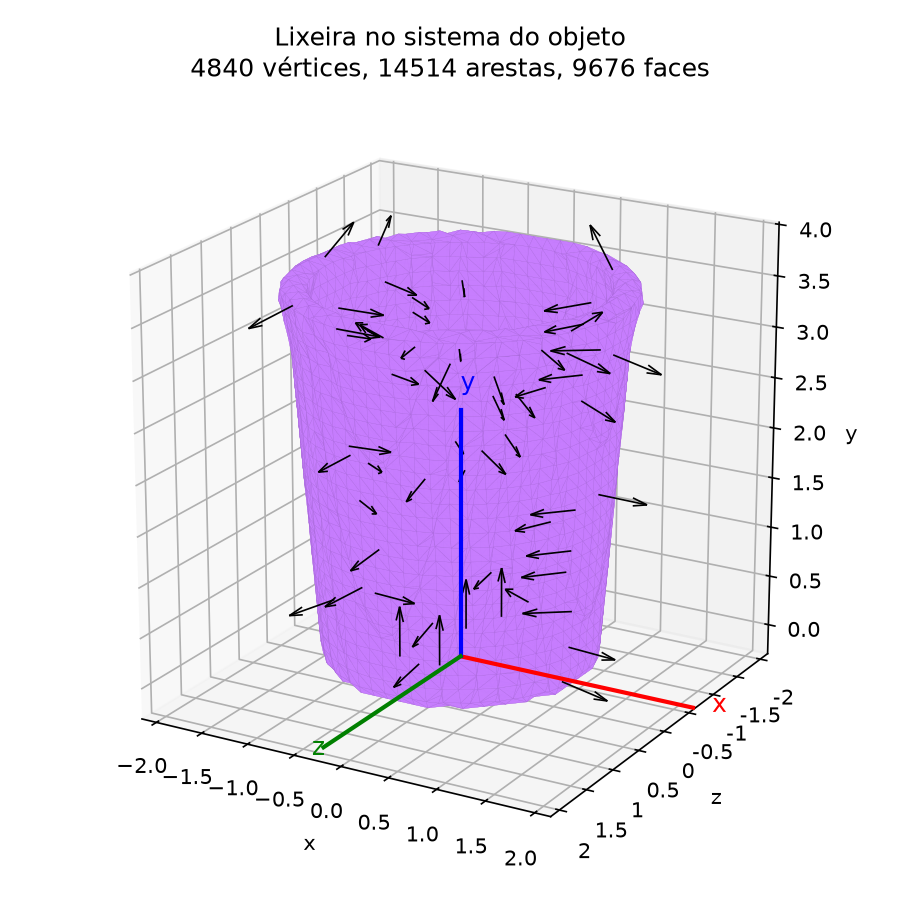
\includegraphics[width=\textwidth]{03-desenvolvimento/01-modelagem/lixeira.png}
    \caption{Lixeira}
  \end{subfigure}
  \fonte{Autoria própria (2026)}
\end{figure}

% Etapa 2 do enunciado: cena no sistema de coordenadas do mundo.
% Fonte no código: math_3d.py (translação, escala, rotações), main.py (CENA)
% Dica: matriz do mundo M = T R S, valores da cena, limite |10|, ausência de interseção.
% Figuras: cena 3D no mundo, em figuras/03-desenvolvimento/02-cena/.
\subsection{Composição da cena}\label{sec:cena}

\confirmar{escrever: transformações aplicadas a cada objeto (escala, rotação, translação) e tabela de posições}

\confirmar{escrever: como foi garantido o limite |10| e a ausência de sobreposição}

% Etapa 3 do enunciado: sistema de coordenadas da câmera.
% Fonte no código: math_3d.py (look_at), main.py (EYE_PRINCIPAL, EYE_BLENDER)
% Dica: eye, at, up, base (u, v, n), matriz de visualização, ponto da origem do mundo,
% mais de um valor de eye gerando novas imagens.
% Figuras: cena no sistema da câmera, em figuras/03-desenvolvimento/03-camera/.
\subsection{Sistema de coordenadas da câmera}\label{sec:camera}

\confirmar{escrever: cálculo da base vetorial a partir de eye, at e up}

\confirmar{escrever: transformação mundo para câmera e marcação da origem do mundo}
\confirmar{escrever: exemplos com valores diferentes de eye}

% Etapa 4 do enunciado: projeção em perspectiva.
% Fonte no código: math_3d.py (projecao_perspectiva, divisao_perspectiva), main.py (ndc_para_pixel)
% Figura do item 4a: visualizar_projecao.py (salva pelo botão de salvar da janela).
\subsection{Projeção em perspectiva}\label{sec:projecao}

Na projeção em perspectiva, objetos mais distantes aparecem menores \cite{azevedo2018}. O volume de
visão é definido pelo ângulo de abertura vertical ($fov = 58^\circ$), pela proporção da janela
($1$) e pelas distâncias dos planos próximo ($0{,}1$) e distante ($100$). Dele sai o valor
$f = \cot(fov/2)$, que corresponde ao $d$ da aula: a posição projetada é

\begin{equation}
  x' = d \cdot \frac{x}{z} .
\end{equation}

Como $z$ está no denominador, quanto mais longe o ponto, mais perto do centro ele fica. No código,
essa conta é feita com uma matriz $4 \times 4$ e uma divisão final pela coordenada $w$. O resultado
são coordenadas entre $-1$ e $1$, que depois são convertidas em pixels da janela de projeção.
Triângulos fora do volume de visão ou voltados para trás não são iluminados nem rasterizados
(Seção~\ref{sec:rasterizacao}). A Figura~\ref{fig:projecao} mostra, à esquerda, os sólidos em 3D
no sistema da câmera com a janela de projeção e, à direita, a janela vista de frente.

\figura{03-desenvolvimento/04-projecao/eye1.png}{\textwidth}{Sólidos em 3D e projeção na janela, com $eye = (9{,}75;\ 13;\ 6{,}5)$}{fig:projecao}{Autoria própria (2026)}

% Etapa 5 do enunciado: iluminação.
% Fonte no código: illumination.py
% Dica: modelo de Phong \cite{phong1975}, componentes ambiente, difusa e especular,
% coeficientes (ka, kd, ks, brilho), posição da luz, cálculo por vértice.
% Figuras: opcional, comparação das componentes, em figuras/03-desenvolvimento/05-iluminacao/.
\subsection{Iluminação}\label{sec:iluminacao}

\confirmar{escrever: equação do modelo de Phong e valores usados}

\confirmar{escrever: como o RGB de cada vértice é calculado}

% Etapa 6 do enunciado: rasterização.
% Fonte no código: rasterizer.py, main.py
% Dica: eliminação de faces ocultas (normal da face e eixo z da câmera), retas (livro-texto,
% subseção 5.2.1), polígonos (par-ímpar com scan line), coordenadas baricêntricas, Z-buffer,
% 3 resoluções.
% Figuras: algoritmo em pseudocódigo ou diagrama, em figuras/03-desenvolvimento/06-rasterizacao/.
\subsection{Rasterização}\label{sec:rasterizacao}

\confirmar{escrever: eliminação de faces ocultas pela normal e pelo eixo z da câmera}

\confirmar{escrever: rasterização de retas e do preenchimento par-ímpar com scan line}

\confirmar{escrever: interpolação baricêntrica da cor e uso do Z-buffer}


% =====================================================================
% 4. Simulações computacionais
% Imagens geradas com o código do projeto (script descartável chamando renderizar_cena_completa).
% Tempos medidos em macOS, Python 3.14, numpy 2.5.5, matplotlib 3.11.2, scikit-image 0.26.0.
% Pendência: refazer as imagens e os tempos se o código do pipeline mudar.
% =====================================================================
\section{Simulações computacionais}\label{sec:simulacoes}

As simulações foram feitas em Python 3.14, com NumPy, Matplotlib e scikit-image. A malha de cada
objeto foi gerada com 80 pontos por eixo. A câmera principal usa $eye = (9{,}75;\ 13;\ 6{,}5)$,
$at = (0, 0, 0)$ e $up = (0, 1, 0)$, e a luz fica em $(5;\ 20;\ 15)$.

\subsection{Três resoluções}\label{sec:sim-resolucoes}

A Figura~\ref{fig:resolucoes} mostra a mesma cena rasterizada em $200 \times 200$, $400 \times 400$
e $800 \times 800$ pixels. Com mais pixels, os contornos ficam mais lisos e o brilho especular
aparece com mais detalhe. Em $200 \times 200$ já dá para reconhecer os objetos, mas as bordas
ficam serrilhadas. O tempo de rasterização foi de 0,8 s, 0,9 s e 1,4 s, respectivamente, sem contar
a geração das malhas, que levou 0,2 s. A cena tem 62\,452 triângulos. Nenhum ficou fora do volume
de visão, 32\,204 foram descartados por estarem de costas e 30\,248 foram desenhados.

\begin{figure}[H]
  \centering
  \caption{Cena rasterizada em três resoluções}\label{fig:resolucoes}
  \begin{subfigure}{0.31\textwidth}
    \centering
    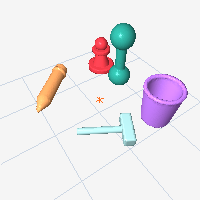
\includegraphics[width=\textwidth]{04-simulacoes/eye1-200.png}
    \caption{$200 \times 200$}
  \end{subfigure}\hfill
  \begin{subfigure}{0.31\textwidth}
    \centering
    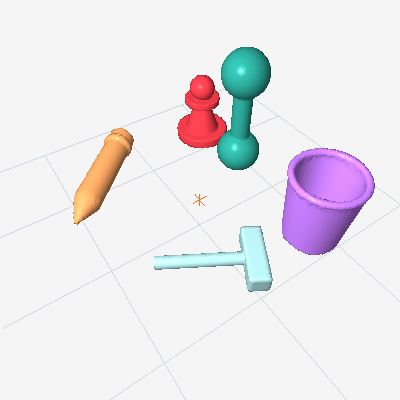
\includegraphics[width=\textwidth]{04-simulacoes/eye1-400.png}
    \caption{$400 \times 400$}
  \end{subfigure}\hfill
  \begin{subfigure}{0.31\textwidth}
    \centering
    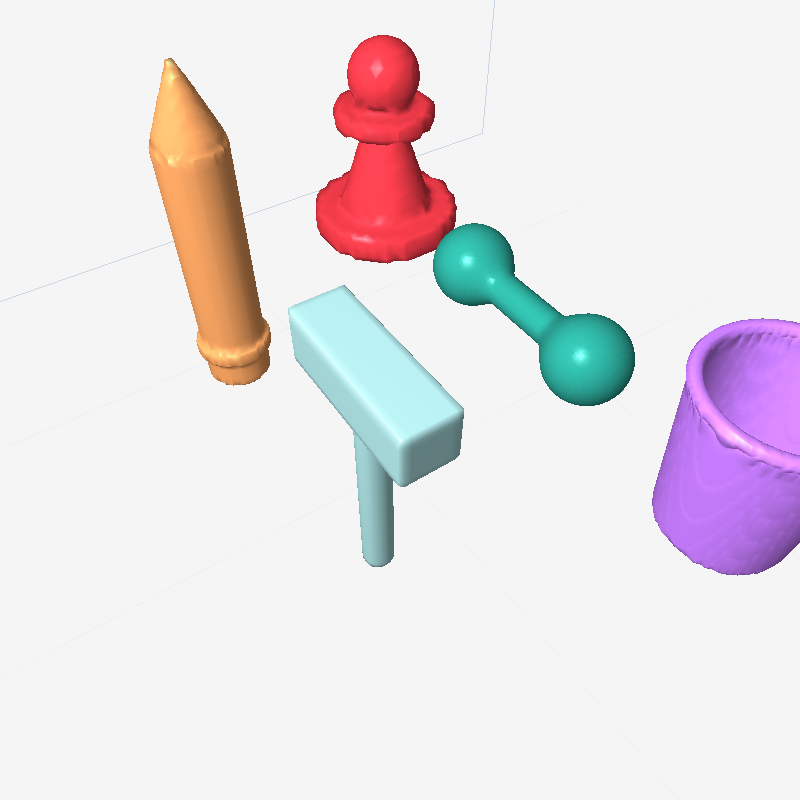
\includegraphics[width=\textwidth]{04-simulacoes/eye1-800.png}
    \caption{$800 \times 800$}
  \end{subfigure}
  \fonte{Os autores (2026).}
\end{figure}

\subsection{Mudança do eye}\label{sec:sim-eye}

Quando o \textit{eye} muda para $(26;\ 18;\ 28)$, o código recalcula a base da câmera e a matriz de
visualização, e a imagem muda. Nessa posição, a câmera fica mais longe e mostra todos os objetos
(Figura~\ref{fig:eye2}).

\figura{04-simulacoes/eye2-400.png}{0.45\textwidth}{Cena vista de $eye = (26;\ 18;\ 28)$, em $400 \times 400$}{fig:eye2}{Os autores (2026)}

% =====================================================================
% 5. Conclusão
% Sem informação nova e sem citação.
% =====================================================================
\section{Conclusão}\label{sec:conclusao}

Neste trabalho, o grupo fez todos os passos para desenhar uma cena 3D na tela. Foram criados cinco
objetos do dia a dia, e cada um virou uma malha de triângulos. Depois, os objetos foram colocados
juntos na cena, vistos por uma câmera, projetados em perspectiva, iluminados e pintados em três
tamanhos de imagem.

Os resultados mostram o que cada passo faz. Mudar o \textit{eye} muda o ponto de vista. A luz dá a
sensação de volume aos objetos. O Z-buffer faz o objeto da frente esconder o de trás. Quanto maior a
imagem, mais lisos ficam os contornos.

Ainda há o que melhorar. Os objetos não foram girados nem aumentados na cena, a lixeira aparece
cortada na câmera principal e o \textit{eye} só muda no código. \confirmar{ajustar esta lista conforme o código final}
Como próximos passos, o usuário poderia escolher o \textit{eye} sem mexer no código, e os polígonos
fora do volume de visão poderiam ser cortados.


% Referências: sem número de seção
\printbibliography[heading=bibintoc,title={Referências}]

\end{document}
